% Created 2017-09-18 Mon 21:40
% Intended LaTeX compiler: pdflatex
\documentclass[setspace, doublespace]{scrartcl}
\usepackage[utf8]{inputenc}
\usepackage[T1]{fontenc}
\usepackage{graphicx}
\usepackage{grffile}
\usepackage{longtable}
\usepackage{wrapfig}
\usepackage{rotating}
\usepackage[normalem]{ulem}
\usepackage{amsmath}
\usepackage{textcomp}
\usepackage{amssymb}
\usepackage{capt-of}
\usepackage{hyperref}
\author{Xiong ChenYu \\
U1521516C \\
EEE \\
}
\date{Sep 18, 2017 \\
}
\title{
\includegraphics[width=\textwidth]{img/NTU.png} \\
[3\baselineskip] PLAN FOR\\
FINAL YEAR PROJECT \\
[6\baselineskip]}
\hypersetup{
 pdfauthor={Xiong ChenYu \\
U1521516C \\
EEE \\
},
 pdftitle={
\includegraphics[width=\textwidth]{img/NTU.png} \\
[3\baselineskip] PLAN FOR\\
FINAL YEAR PROJECT \\
[6\baselineskip]},
 pdfkeywords={},
 pdfsubject={},
 pdfcreator={Emacs 27.0.50 (Org mode 9.1)},
 pdflang={English}}
\begin{document}

\maketitle
\tableofcontents

\listoffigures

\usepackage{indentfirst}
\newpage
\section{Background}
\label{sec:org095b14e}

With the progress of the technology, there are more and more share Economy types come into being.
Suck as share-bicycle, share-powerbank etc.

The delivery service in Singapore is expensive. One possible solution is to build self-collection spot.
But the land price is very high it is unreliable to build the collection spot everywhere.

So I come up with this idea to fit-fight delivery. One person can volunteer as the leader,
and he will be response as an dynamic collection spot to let the other member to collect the
goods at his place and he can also benefit to get free delivery.
And from providing this kind of service we can also learn what people want to buy from
outside of Singapore.

\section{My final year project plan}
\label{sec:org8d82581}
This project will use modern technology to build a security high performance type safe international delivery sharing management system to fit fight group, deliver, track, and notify the receiver using functional programming to meet the modern share economy requirements.

The website consist of 3 part. The portal for end user to request for delivering join or start a fit fight group. The backend management system for logistics company to check and confirm. A list of Api for logistics company to update the delivering info.

And a helper system to help analyzing the marketing with the modern data mining and ai technology. The Logistics can use the system to analyse the customers behavior, predict the packages distribution and floating the price base on the market to get the highest profit for logistics company. Moreover, the local e-commerce can get the latest market analyze and adapt to meet the requirements of the rapidly changing market.

This project will find and cooperate with the international logistic company for data source and ai model training.

\section{My strategy}
\label{sec:orgde7f2c2}

For the web part I am going to use the Nodejs to build the web server and use purescript to write the front end.

I am going to start the machine learning part in the holiday cause the data I collect is not enough.

\section{Gantt Table}
\label{sec:orgd625beb}
\begin{verbatim}
Project starts the 18th of Sep 2017
[Research and Learn] lasts 31 days and is colored in Lavender/LightBlue
[Prototype Design] lasts 31 days and is colored in Coral/Green
[Prototype Design] starts 14 days after [Research and Learn]'s end
[Test prototype] lasts 31 days and is colored in Red
[Test prototype] starts 2 days before [Prototype Design]'s end
[Write tests] lasts 5 days and ends at [Prototype Design]'s end
[Document] lasts 31 days and ends at [Write tests]'s start
[Init and write tests report] is colored in Coral/Green
[Init and write tests report] starts 31 day after [Test prototype]'s start
\end{verbatim}

\begin{figure}[htbp]
\caption{\label{fig:orgb0a6ab5}
Gantt Table}
\centering
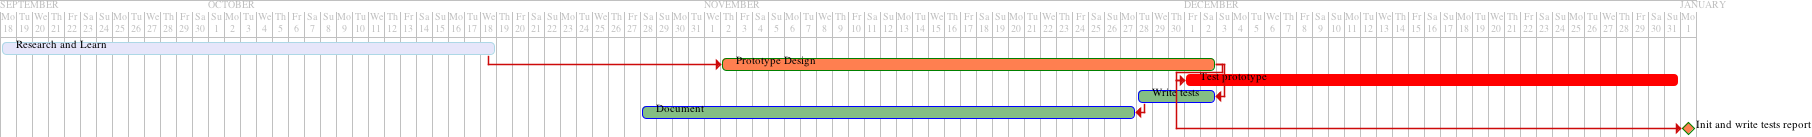
\includegraphics[width=.9\linewidth]{img/gantt.png}
\end{figure}
\end{document}